\documentclass{standalone}
\usepackage{tikz}
\usepackage{amsmath,dsfont}
\usetikzlibrary{automata,positioning,arrows,shapes.geometric, calc,patterns}

\begin{document}
	%	\begin{tikzpicture}[
		%		shaded/.style={draw,circle,pattern=north east lines, pattern color=yellow},
		%		> = stealth',
		%		auto,
		%		prob/.style = {inner sep=1pt,font=\footnotesize}
		%		]
		%		% Markov Chain
		%		\node[shaded] at (0,0) (s1) {$s_1$};
		%		\node[shaded, right= of s1] (s2) {$s_2$};
		%		% Draw the causality arrows
		%		\path[->] 	(s1) edge [loop left] node[prob] {$0.1$}(s1)
		%		(s2) edge [loop right] node[prob] {$0.2$}(s2)
		%		(s1) edge [bend left=10] node[prob]{$0.9$} (s2)
		%		(s2) edge [bend left = 10] node[prob] {$0.8$}(s1);
		%		
		%		% denote
		%		\node[above = of s1,align=center,xshift= 10mm,yshift = -4mm] (S){ $\mathds{S} = \{s_1,s_2\}$,$\mathbf{T} = \mathbf{T}(s)$ };
		%		
		%		\node[above = of S,align=center,xshift= 1mm,yshift = -4mm]  {Markov Chain: $2-$tuple $(\mathds{S},\mathbf{T})$};
		%		%\node[above = of s1,align=center,xshift= 1mm,yshift = -4mm]  {Markov Chain};
		%		\node[below = of s1,align=center,xshift= 8mm,yshift = 4mm] (TP)  { Transition Model: $\pi(s'|s)$, for discrete states are  transition matrix \\$
			%			\mathbf{T} = [\pi(s'|s)] =
			%			\begin{array}{cc}
				%				& \begin{array}{cc} s_1 & s_2 \end{array} \\
				%				\begin{array}{c}
					%					s_1 \\
					%					s_2 \\
					%				\end{array}
				%				& \left[ \begin{array}{cc}
					%					0.1 & 0.9 \\
					%					0.8 & 0.2  \\
					%				\end{array} \right]
				%			\end{array}
			%			$};
		%		\node[below= of TP,align=center,xshift= 0mm,yshift = 5mm] (observation) {Sensor Model: States are completely observable\\i.e. $p(o_1|s_1) = 1$, $p(o_2|s_2) = 1$};	
		%		%	\node[below= of TP,align=center,xshift= 0mm,yshift = 5mm] (next) {$\pi(s'|s)$: };
		%		
		%	\end{tikzpicture}
	%	
	%	% Hidden Markov Model
	%	\begin{tikzpicture}[
		%		shaded/.style={draw,circle,pattern=north east lines, pattern color=yellow},
		%		> = stealth',
		%		auto,
		%		prob/.style = {inner sep=1pt,font=\footnotesize}
		%		]
		%		\node[shaded] at (0,0) (s1) {$s_1$};
		%		\node[shaded, right= of s1] (s2) {$s_2$};
		%		% Draw the causality arrows
		%		\path[->] 	(s1) edge [loop left] node[prob] {$0.1$}(s1)
		%		(s2) edge [loop right] node[prob] {$0.2$}(s2)
		%		(s1) edge [bend left=10] node[prob]{$0.9$} (s2)
		%		(s2) edge [bend left = 10] node[prob] {$0.8$}(s1);
		%		
		%		% denote
		%		%\node[above = of s1,align=center,xshift= 1mm,yshift = -4mm]  {Hidden Markov Model};
		%		\node[above = of s1,align=center,xshift= 10mm,yshift = -4mm] (S){ $\mathds{S} = \{s_1,s_2\}$, $\mathds{O} = \{o_1,o_2\}$, $\mathbf{T} = \mathbf{T}(s)$, $\mathbf{O} = \mathbf{O}(o|s')$};
		%		
		%		\node[above = of S,align=center,xshift= 1mm,yshift = -4mm]  {Hidden Markov Model: $4-$tuple $(\mathds{S},\mathds{O},\mathbf{T},\mathbf{O})$};
		%		
		%		\node[below = of s1,align=center,xshift= 8mm,yshift = 4mm] (TP)  { Transition Model: $\pi(s'|s)$, for discrete states are  transition matrix \\ $ 
			%			\mathbf{T} = [\pi(s'|s)] =
			%			\begin{array}{cc}
				%				& \begin{array}{cc} s_1 & s_2 \end{array} \\
				%				\begin{array}{c}
					%					s_1 \\
					%					s_2 \\
					%				\end{array}
				%				& \left[ \begin{array}{cc}
					%					0.1 & 0.9 \\
					%					0.8 & 0.2  \\
					%				\end{array} \right]
				%			\end{array}
			%			$};
		%		%	\node[below= of TP,align=center,xshift= 0mm,yshift = 5mm] (next) {$\pi(s'|s)$: Next state $s'$ is determined \\ only by the current state $s$};
		%		\node[below= of TP,align=center,xshift= 0mm,yshift = 5mm] (next) {Sensor Model: $\mathbf{O} = \mathbf{O}(o|s)$ \\We are unsure which state we are in \\e.g. $p(o_1|s_1) = 0.75$, $p(o_2|s_2) = 0.75$};	
		%	\end{tikzpicture}
	%	
	%	% Markov Decision Process
	%	\begin{tikzpicture}[
		%		shaded/.style={draw,circle,pattern=north east lines, pattern color=yellow},
		%		> = stealth',
		%		auto,
		%		prob/.style = {inner sep=1pt,font=\footnotesize}
		%		]
		%		\node[shaded] at (0,0) (s1) {$s_1$};
		%		\node[shaded, right= of s1,xshift= 8mm] (s2) {$s_2$};
		%		% Draw the causality arrows
		%		\path[->] 	
		%		(s1) edge [loop left,blue] node[prob] {$a_1 0.3$}(s1)
		%		(s1) edge [loop below,brown,dashed] node[prob] {$a_2 0.1$}(s1)
		%		(s2) edge [loop right,blue] node[prob] {$a_1 0.4$}(s2)
		%		(s2) edge [loop below,brown,dashed] node[prob] {$a_2 0.2$}(s2)
		%		(s1) edge [bend left=10,blue] node[prob]{$a_1 0.7$} (s2)
		%		(s1) edge [bend left = 40,brown,dashed] node[prob]{$a_2 0.9$} (s2)
		%		(s2) edge [bend left = 10,blue] node[prob] {$a_1 0.6$}(s1)
		%		(s2) edge [bend left = 40,brown,dashed] node[prob] {$a_2 0.8$}(s1);
		%		
		%		% denote
		%		\node[above = of s1,align=center,xshift= 10mm,yshift = -4mm] (S){ $\mathds{S} = \{s_1,s_2\}$, $\mathds{A} = \{a_1,a_2\}$,
			%			$\mathbf{T} = \mathbf{T}(s,a)$, $\mathbf{r} = \mathbf{r}(s,a)$ };
		%		
		%		\node[above = of S,align=center,xshift= 1mm,yshift = -4mm]  {Markov Decision Process: $4-$tuple $(\mathds{S},\mathds{A},\mathbf{T},\mathbf{r})$};
		%		
		%		\node[below = of s1,align=center,xshift= 8mm,yshift = 4mm] (TP)  { Transition Model: $\pi(s'|s,a)$, for discrete states are transition matrix \\$
			%			\mathbf{T}  = [\pi(s'|s,a)] = 
			%			\begin{array}{ccc}
				%				&  &\begin{array}{cc} s_1 & s_2 \end{array} \\
				%				\begin{array}{c}
					%					s_1 \\
					%					s_2 
					%				\end{array} 
				%				&
				%				\begin{array}{c}
					%					\textcolor{blue}{a_1} \\
					%					\textcolor{brown}{a_2} \\
					%					\textcolor{blue}{a_1} \\
					%					\textcolor{brown}{a_2}
					%				\end{array} 
				%				& \left[ \begin{array}{cc}
					%					\textcolor{blue}{a_1}& \textcolor{blue}{0.7}\\
					%					\textcolor{brown}{0.1} & \textcolor{brown}{0.9} \\
					%					\textcolor{blue}{0.6} & \textcolor{blue}{0.4} \\
					%					\textcolor{brown}{0.8} & \textcolor{brown}{0.2}  
					%				\end{array} \right]
				%			\end{array}
			%			$};
		%		%	\node[below= of TP,align=center,xshift= 0mm,yshift = 5mm] (next) { $\pi(s'|s,a)$: Next state $s'$ is determined by \\ current state $s$ and current action $a$};
		%		\node[below = of TP,align=center,xshift= 0mm,yshift = 4mm] (reward)  { Reward Model $r(s,a)$ or $r(s,a,s')$ \\$
			%			\mathbf{r}  = [r(s,a,s')] =
			%			\begin{array}{ccc}
				%				&  &\begin{array}{cc} s_1 & s_2 \end{array} \\
				%				\begin{array}{c}
					%					s_1 \\
					%					s_2 
					%				\end{array} 
				%				&
				%				\begin{array}{c}
					%					a_1 \\
					%					a_2 \\
					%					a_1 \\
					%					a_2
					%				\end{array} 
				%				& \left[ \begin{array}{cc}
					%					r_{111} & r_{112} \\
					%					r_{121} & r_{122} \\
					%					r_{211} & r_{212}\\
					%					r_{221} & r_{222} 
					%				\end{array} \right]
				%			\end{array}
			%			$};
		%		\node[below= of reward,align=center,xshift= 0mm,yshift = 5mm] (next) {Sensor Model. States are completely observable\\i.e. $p(o_1|s_1) = 1$, $p(o_2|s_2) = 1$};	
		%	\end{tikzpicture}
	%	
	% Discrete Time Markov Decision Process
	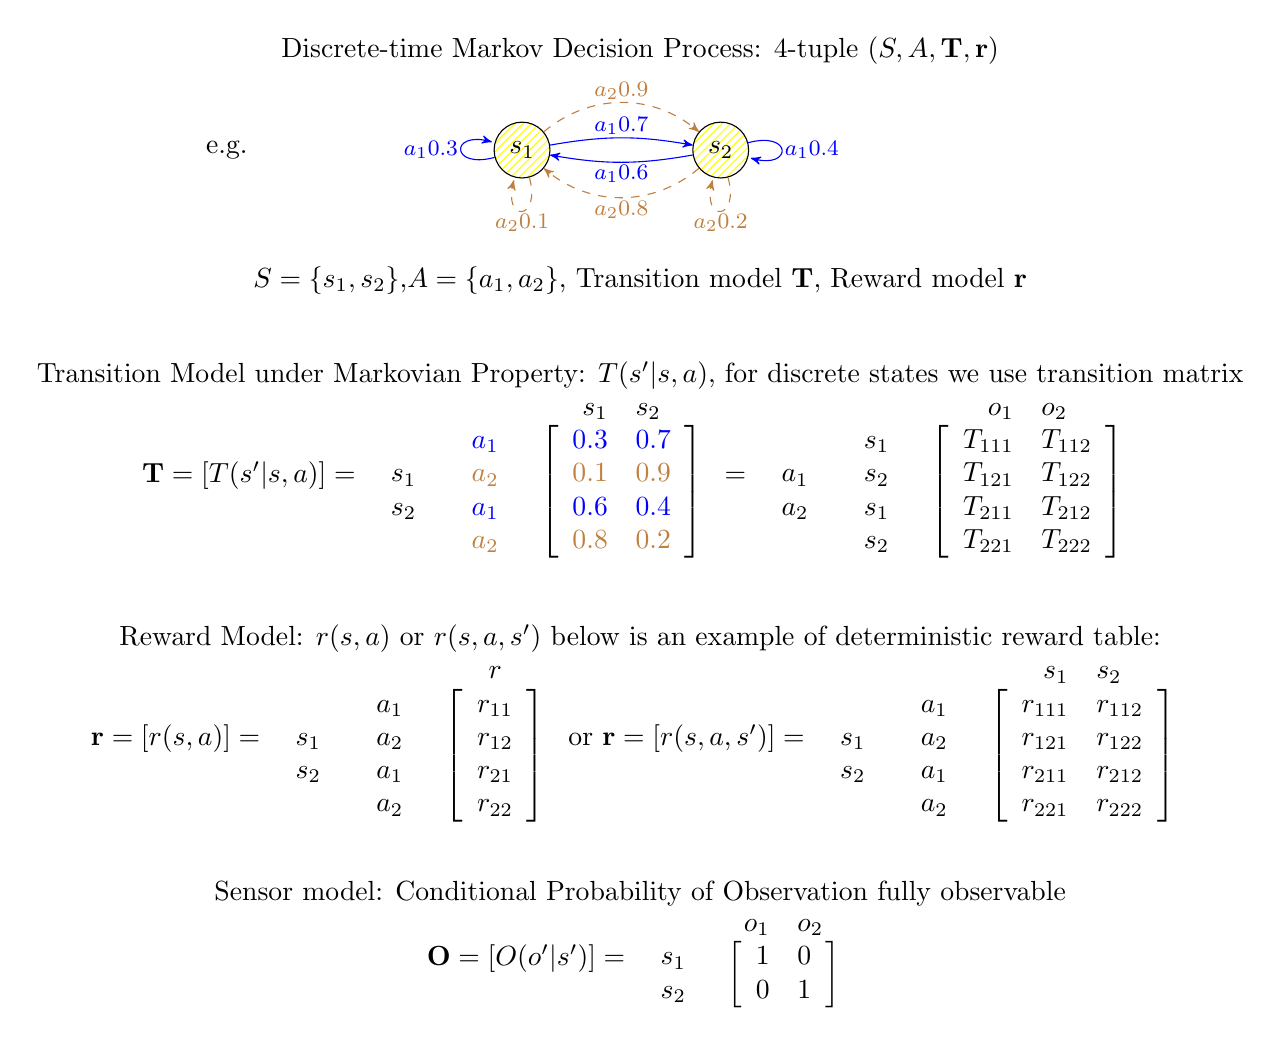
\begin{tikzpicture}[
		shaded/.style={draw,circle,pattern=north east lines, pattern color=yellow},
		> = stealth',
		auto,
		prob/.style = {inner sep=1pt,font=\footnotesize}
		]
		\node[shaded] at (0,0) (s1) {$s_1$};
		\node[shaded, right= of s1,xshift= 8mm] (s2) {$s_2$};
		% Draw the causality arrows
		\path[->] 	
		(s1) edge [loop left,blue] node[prob] {$a_1 0.3$}(s1)
		(s1) edge [loop below,brown,dashed] node[prob] {$a_2 0.1$}(s1)
		(s2) edge [loop right,blue] node[prob] {$a_1 0.4$}(s2)
		(s2) edge [loop below,brown,dashed] node[prob] {$a_2 0.2$}(s2)
		(s1) edge [bend left=10,blue] node[prob]{$a_1 0.7$} (s2)
		(s1) edge [bend left = 40,brown,dashed] node[prob]{$a_2 0.9$} (s2)
		(s2) edge [bend left = 10,blue] node[prob] {$a_1 0.6$}(s1)
		(s2) edge [bend left = 40,brown,dashed] node[prob] {$a_2 0.8$}(s1);
		% 
		\node[left = of s1, xshift = -20mm]{e.g.};
		% denote
		\node[below = of s1,align=center,xshift= 15mm,yshift = 0mm](S)  {$\mathds{S} = \{s_1,s_2\}$,$\mathds{A} = \{a_1,a_2\}$, Transition model $\mathbf{T}$, Reward model $\mathbf{r} $};
		\node[above = of s1,align=center,xshift= 15mm,yshift = -4mm]  {Discrete-time Markov Decision Process: 4-tuple $(\mathds{S},\mathds{A},\mathbf{T},\mathbf{r})$};
		\node[below = of S,align=center,xshift= 0mm,yshift = 4mm] (TP)  { Transition Model under Markovian Property: $T(s'|s,a)$, for discrete states we use transition matrix \\$
			\mathbf{T}  = [T(s'|s,a)] =
			\begin{array}{ccc}
				& &\begin{array}{cc} s_1 & s_2 \end{array} \\
				\begin{array}{c}
					s_1 \\
					s_2 
				\end{array} 
				&
				\begin{array}{c}
					\textcolor{blue}{a_1} \\
					\textcolor{brown}{a_2} \\
					\textcolor{blue}{a_1} \\
					\textcolor{brown}{a_2}
				\end{array} 
				& \left[ \begin{array}{cc}
					\textcolor{blue}{0.3} & \textcolor{blue}{0.7} \\
					\textcolor{brown}{0.1} & \textcolor{brown}{0.9} \\
					\textcolor{blue}{0.6} & \textcolor{blue}{0.4} \\
					\textcolor{brown}{0.8} & \textcolor{brown}{0.2}  
				\end{array} \right]
			\end{array} = 			\begin{array}{ccc}
				&  &\begin{array}{cc} o_1 & o_2 \end{array} \\
				\begin{array}{c}
					a_1 \\
					a_2 
				\end{array} 
				&
				\begin{array}{c}
					s_1 \\
					s_2 \\
					s_1 \\
					s_2
				\end{array} 
				& \left[ \begin{array}{cc}
					T_{111} & T_{112} \\
					T_{121} & T_{122} \\
					T_{211} & T_{212}\\
					T_{221} & T_{222} 
				\end{array} \right]
			\end{array}
			$};
		%	\node[below= of TP,align=center,xshift= 0mm,yshift = 5mm] (next) { $\pi(s'|s,a)$: Next state $s'$ is determined by \\ current state $s$ and current action $a$};
		\node[below = of TP,align=center,xshift= 0mm,yshift = 4mm] (reward)  {Reward Model: $r(s,a)$ or $r(s,a,s')$ below is an example of deterministic reward table: \\$
			\mathbf{r}  = [r(s,a)] =
			\begin{array}{ccc}
				& &\begin{array}{c} r \end{array} \\
				\begin{array}{c}
					s_1 \\
					s_2 
				\end{array} 
				&
				\begin{array}{c}
					a_1 \\
					a_2 \\
					a_1 \\
					a_2
				\end{array} 
				& \left[ \begin{array}{c}
					r_{11} \\
					r_{12} \\
					r_{21} \\
					r_{22} 
				\end{array} \right]
			\end{array}
			$ or 
			$
			\mathbf{r}  = [r(s,a,s')] =
			\begin{array}{ccc}
				&  &\begin{array}{cc} s_1 & s_2 \end{array} \\
				\begin{array}{c}
					s_1 \\
					s_2 
				\end{array} 
				&
				\begin{array}{c}
					a_1 \\
					a_2 \\
					a_1 \\
					a_2
				\end{array} 
				& \left[ \begin{array}{cc}
					r_{111} & r_{112} \\
					r_{121} & r_{122} \\
					r_{211} & r_{212}\\
					r_{221} & r_{222} 
				\end{array} \right]
			\end{array}
			$};
		\node[below= of reward,align=center,xshift= 0mm,yshift = 5mm] (next) {Sensor model: Conditional Probability of Observation
		fully observable\\$
			\mathbf{O}  = [O(o'|s')] =
			\begin{array}{cc}
				&\begin{array}{cc} o_1 & o_2 \end{array} \\
				\begin{array}{c}
					s_1 \\
					s_2 
				\end{array} 
				& \left[ \begin{array}{cc}
					1 & 0 \\
					0 & 1 \\
				\end{array} \right]
			\end{array}
			$
		};	
	\end{tikzpicture}
	
	
	
\end{document}
